\documentclass[conference]{IEEEtran}
\IEEEoverridecommandlockouts

% ---- Codificación e idioma ----
\usepackage[utf8]{inputenc}
\usepackage[T1]{fontenc}
\usepackage[spanish,es-noshorthands]{babel}

% ---- Paquetes ----
\usepackage{graphicx}
\usepackage{amsmath,amssymb}
\usepackage{booktabs}
\usepackage{array}
\usepackage{textcomp}
\usepackage{url}
\usepackage{xcolor}
\usepackage[hidelinks]{hyperref}

\graphicspath{{../docs/img/}{./}}

% Evita "underfull/overfull" agresivos en doble columna
\sloppy

\begin{document}

\title{IRONMAN: un asistente ``Jarvis'' local en CPU\\
\large Cuantización, KV cache, RAG y herramientas MCP}

\author{\IEEEauthorblockN{Guillermo Paredes}
\IEEEauthorblockA{\textit{Applied Machine Learning: Local LLM Systems}\\
guillermouide@gmail.com}}

\maketitle

% ============================ ABSTRACT ============================
\begin{abstract}
Presentamos IRONMAN, un asistente personal tipo ``Jarvis'' que corre
íntegramente en la CPU de un portátil con menos de 16~GB de RAM, sin ningún
LLM en la nube. El sistema combina un modelo \texttt{llama3.2} de 3B
parámetros servido por Ollama, un pipeline RAG local
(\texttt{nomic-embed-text} + \texttt{sqlite-vec}) sobre $\sim$202 páginas de
documentación técnica, y seis herramientas expuestas mediante un servidor
propio del \emph{Model Context Protocol} (MCP), incluyendo correo IMAP/SMTP y
control del PC. La interfaz principal es de texto (\texttt{asistente/jarvis.py}).
Medimos el efecto de tres niveles de cuantización (Q8\_0, Q4\_K\_M, Q3\_K\_M)
sobre tamaño, RAM y velocidad; verificamos el crecimiento aproximadamente
lineal del KV cache entre 512 y 16\,384 tokens de contexto y el ahorro de
cuantizarlo a Q8; y evaluamos el sistema completo con un test set reproducible
de 21 prompts en cinco categorías. El hallazgo principal: Q4\_K\_M es el mejor
compromiso ($\sim$1.7$\times$ más tokens/s que Q8\_0 con idéntica calidad,
2.4/3); en estas 5 pruebas las tres cuantizaciones empatan en 2.4/3, así que la
elección Q4 frente a Q3 se apoya en el margen de fiabilidad, no en la calidad
medida. El KV cache crece $\sim$117~KB/token, casi los 112~KB/token teóricos,
confirmando su crecimiento lineal con el contexto.
\end{abstract}

\begin{IEEEkeywords}
LLM local, cuantización, KV cache, RAG, Model Context Protocol, inferencia en
CPU, Ollama.
\end{IEEEkeywords}

% ============================ ARQUITECTURA ============================
\section{Arquitectura del sistema}

\begin{figure}[t]
\centering
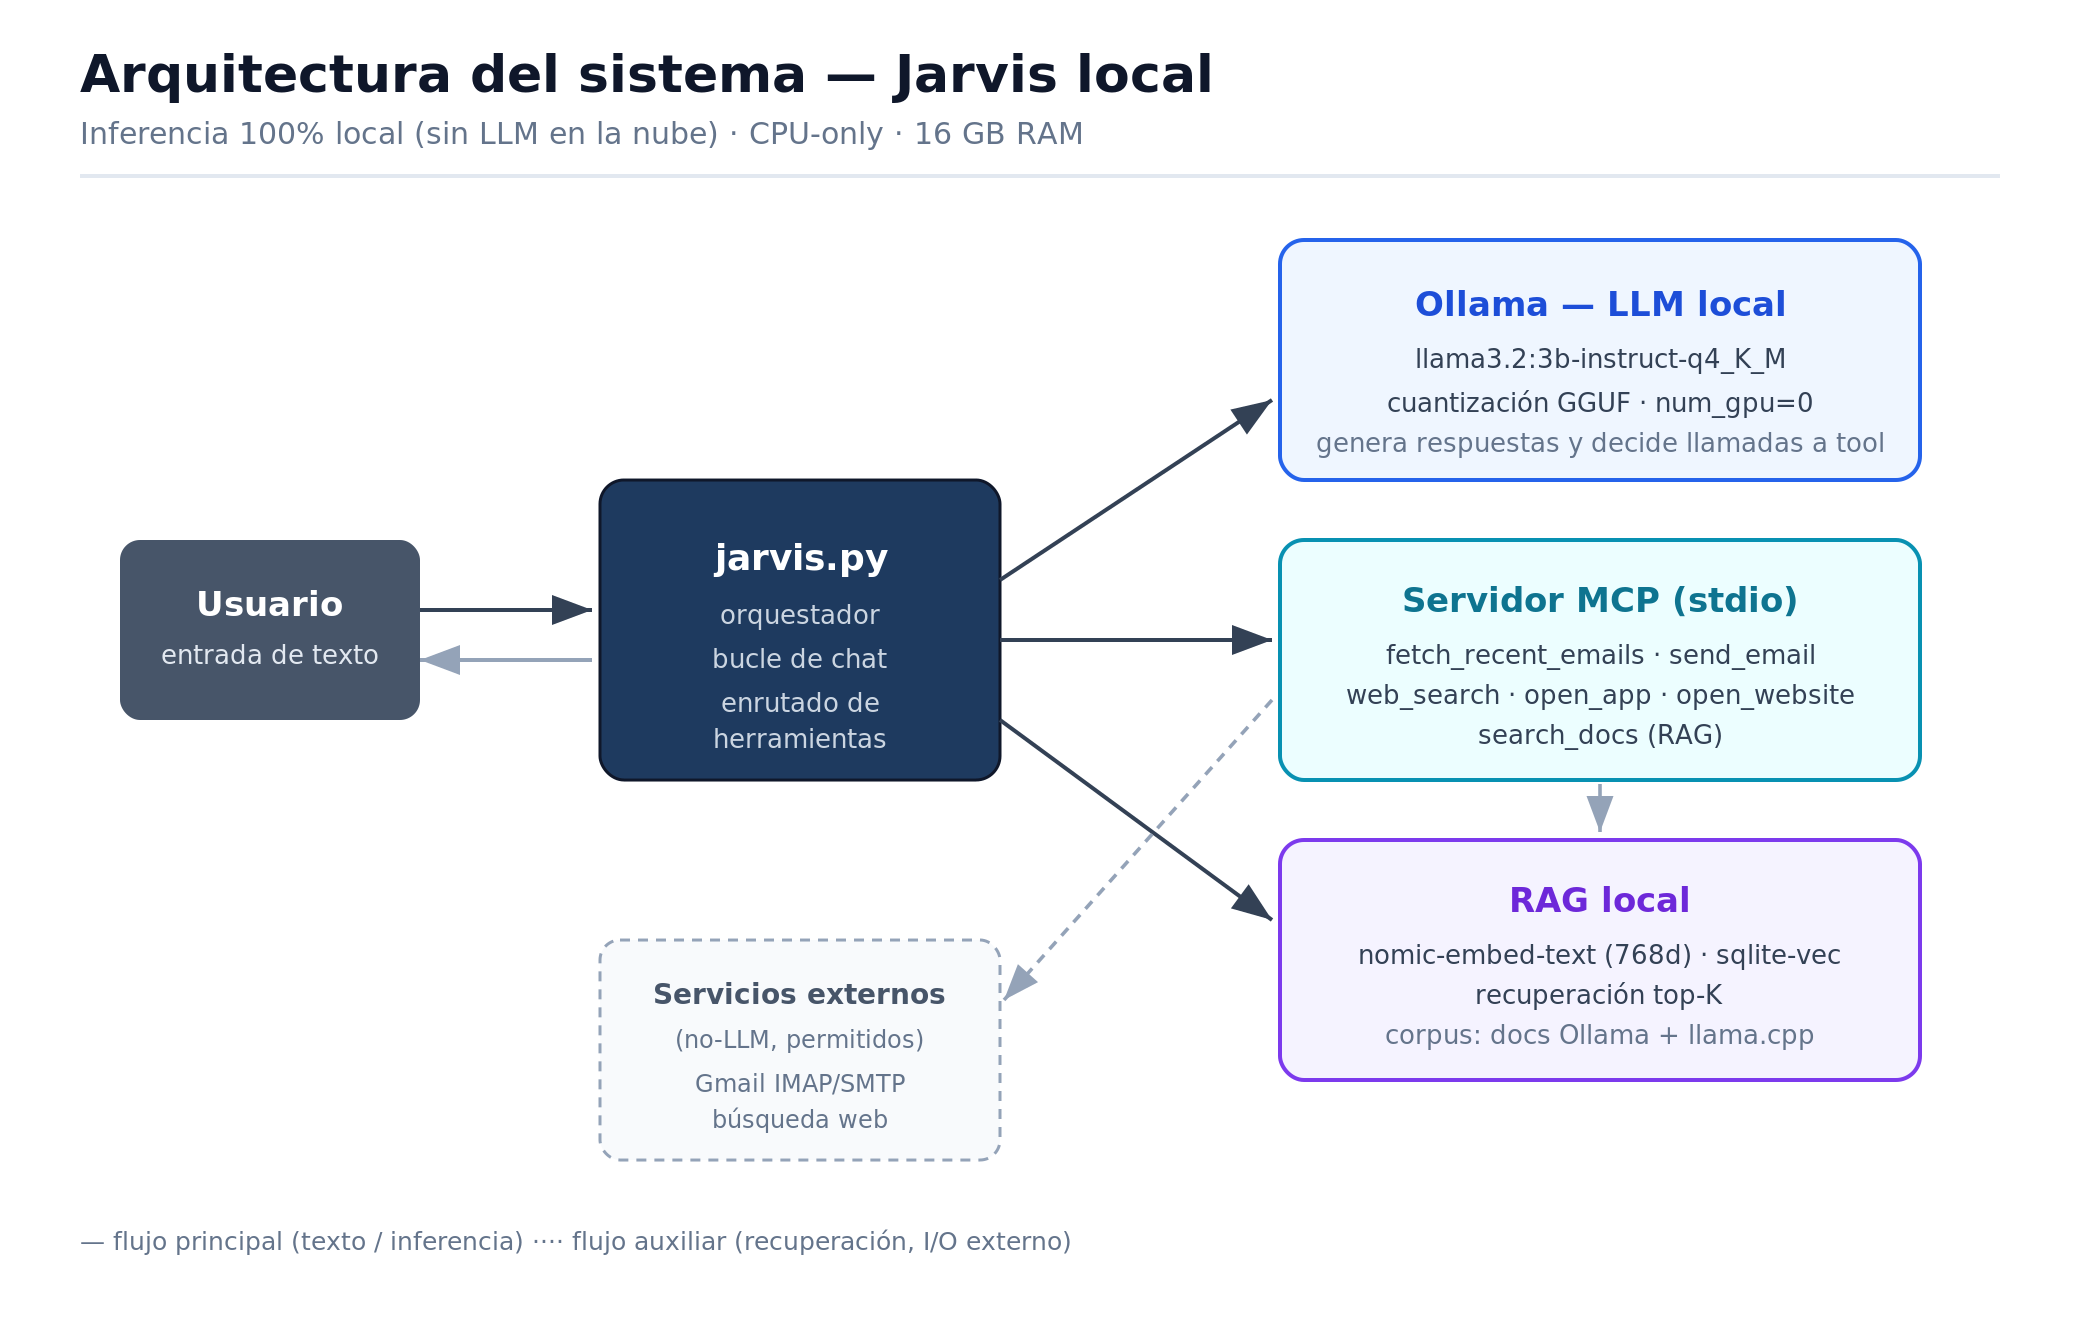
\includegraphics[width=\columnwidth]{arquitectura.png}
\caption{Arquitectura general. El usuario interactúa por texto con
\texttt{jarvis.py}, que orquesta la inferencia local (Ollama), la llamada a
herramientas (MCP) y la recuperación (RAG). Ningún componente de inferencia
sale a la nube.}
\label{fig:arq}
\end{figure}

La interfaz del núcleo es de texto (\texttt{asistente/jarvis.py}), la misma que
usa la evaluación automática de la Parte E. Todas las llamadas de inferencia
fijan \texttt{num\_gpu:~0}: el equipo tiene una RTX~4060 que se deshabilita
explícitamente para cumplir la restricción de hardware del enunciado.

El servidor MCP propio (\texttt{asistente/mcp\_server.py}) expone seis
herramientas por stdio: \texttt{fetch\_recent\_emails} y \texttt{send\_email}
(Gmail IMAP/SMTP), \texttt{open\_app}, \texttt{open\_website} y
\texttt{web\_search} (control del PC y búsqueda), y \texttt{search\_docs}
(puente al RAG sobre el top-4 de 1134 chunks del corpus de docs de Ollama y
llama.cpp, $\sim$202 págs).

\begin{figure}[t]
\centering
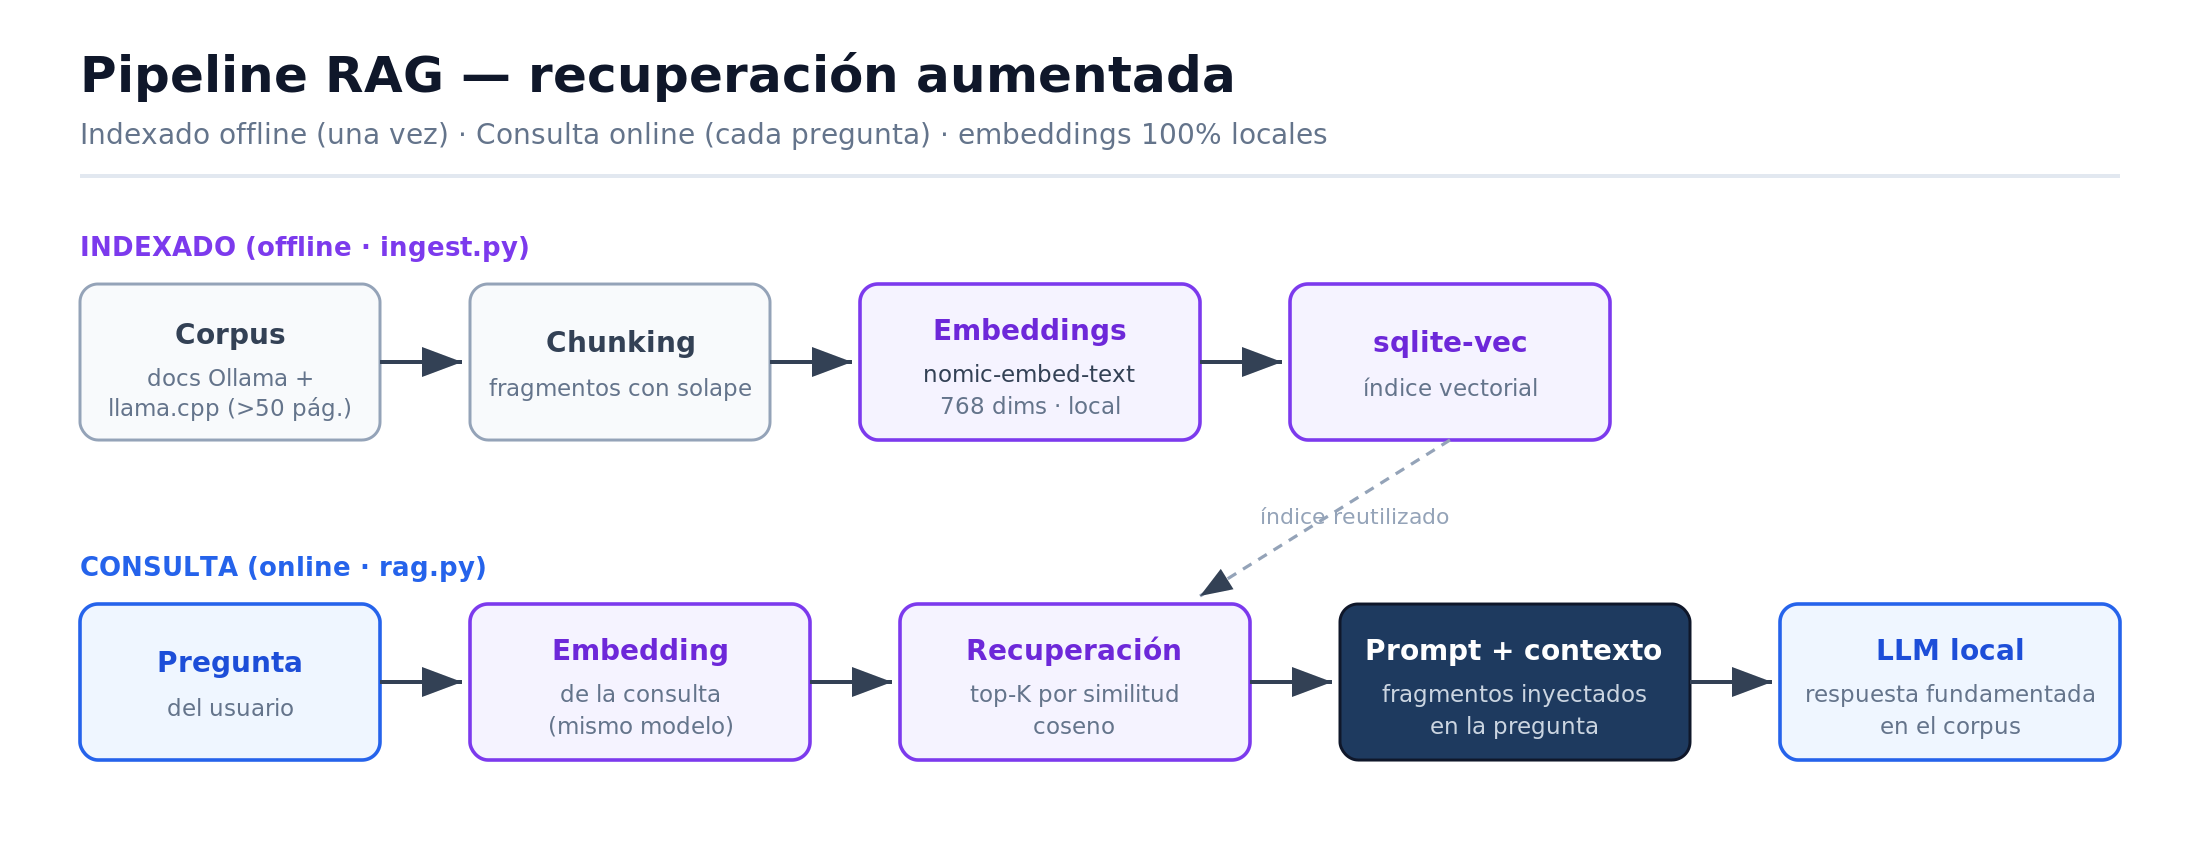
\includegraphics[width=\columnwidth]{flujo_rag.png}
\caption{Pipeline RAG. El indexado (offline, \texttt{parte\_c\_rag.py ingest})
trocea el corpus, lo incrusta con \texttt{nomic-embed-text} y lo guarda en
\texttt{sqlite-vec}. En consulta (online) la pregunta se incrusta con el mismo
modelo, se recuperan los top-$K$ fragmentos por similitud coseno y se inyectan
en el prompt.}
\label{fig:rag}
\end{figure}

\begin{figure}[t]
\centering
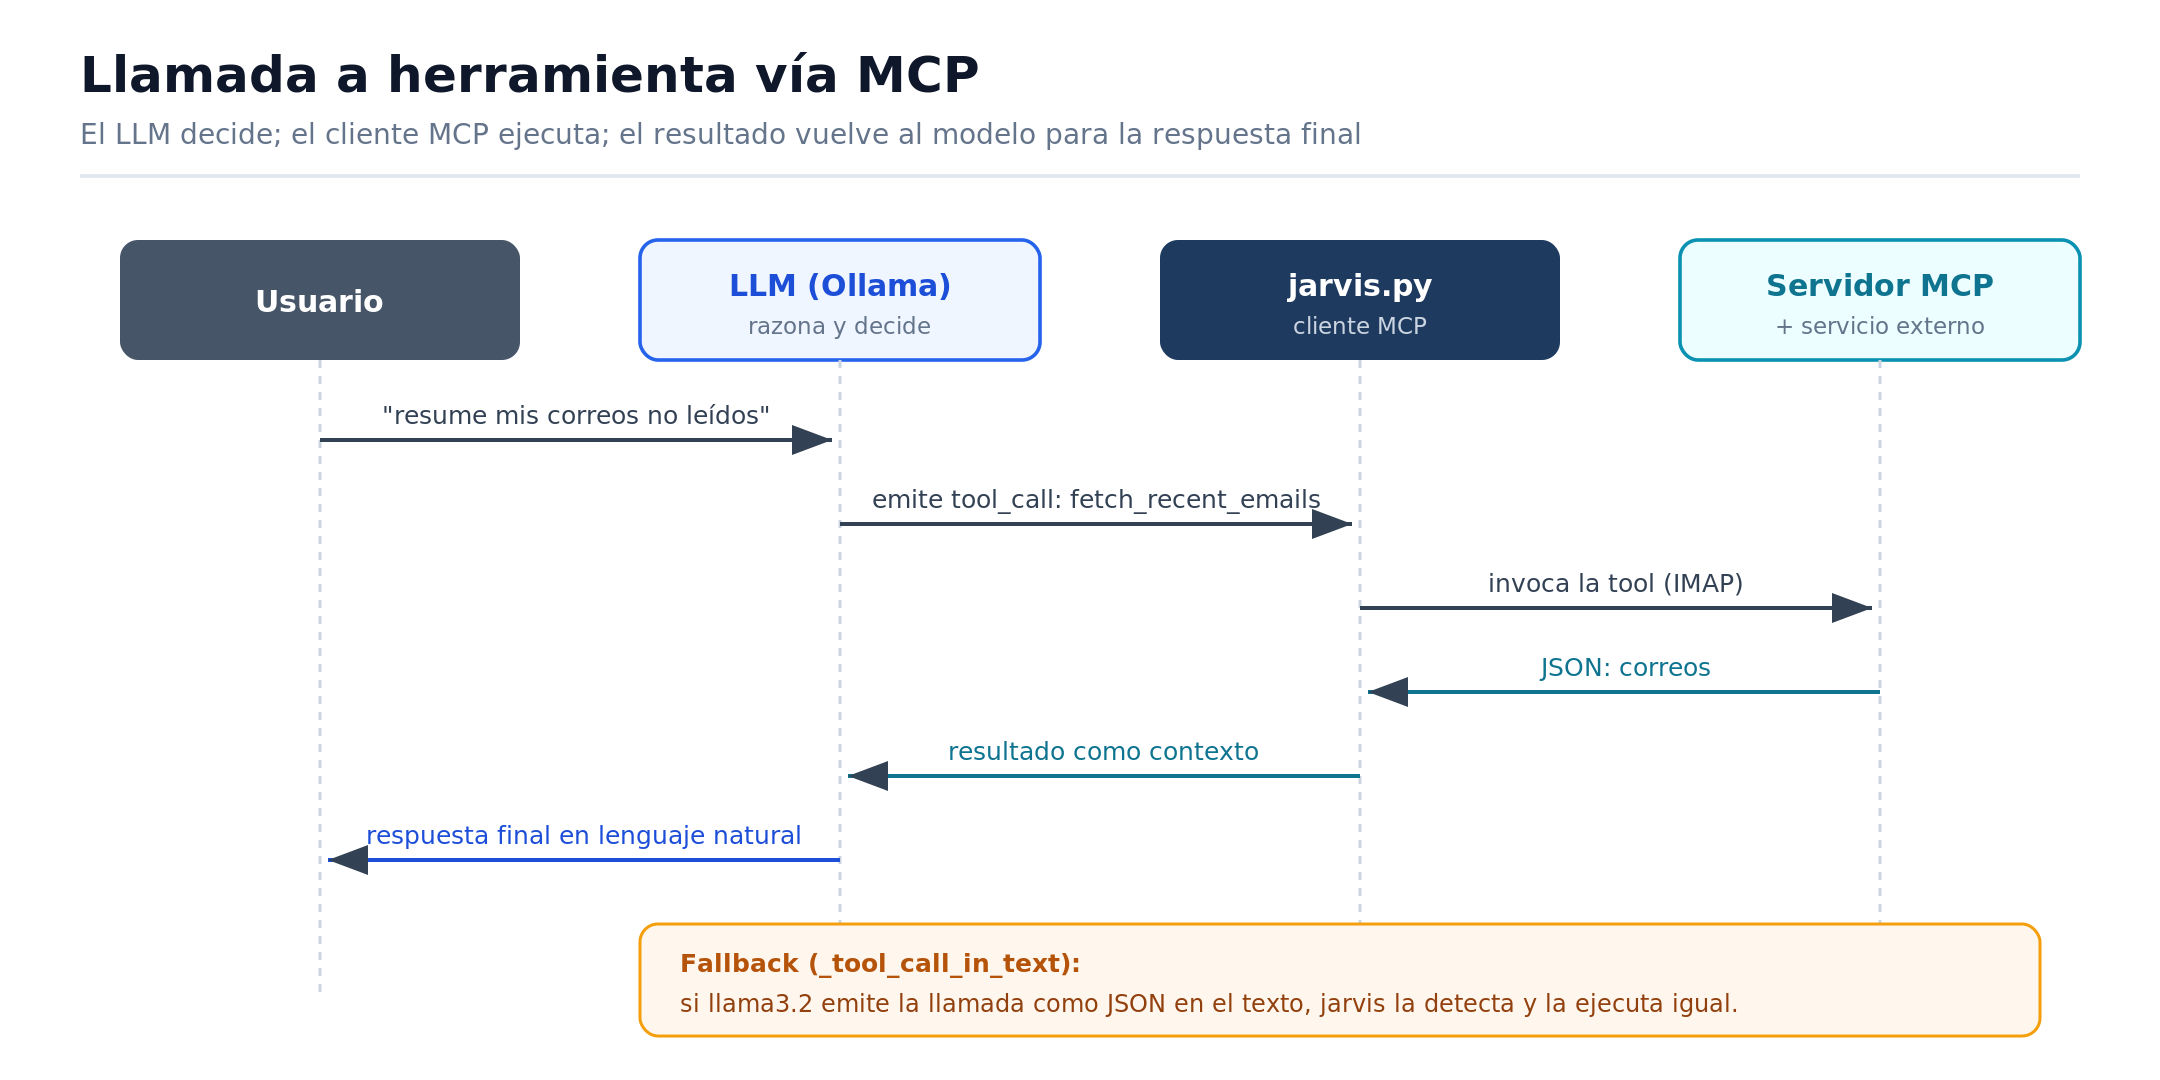
\includegraphics[width=\columnwidth]{flujo_mcp.png}
\caption{Secuencia de una llamada a herramienta. El LLM emite un
\texttt{tool\_call}, el cliente MCP de \texttt{jarvis.py} ejecuta la herramienta
en el servidor, y el resultado vuelve al modelo como contexto para la respuesta
final. El fallback \texttt{\_tool\_call\_in\_text} captura los casos en que
\texttt{llama3.2} emite la llamada como JSON dentro del texto.}
\label{fig:mcp}
\end{figure}

% ============================ METODOLOGÍA ============================
\section{Metodología}

\textbf{Hardware.} ASUS ROG Strix G614JV: Intel i7-13650HX (14 núcleos /
20 hilos), 15.6~GB RAM, Windows~11. GPU dedicada deshabilitada por software
(\texttt{num\_gpu:~0} en cada petición; verificado observando 0~MB de VRAM en
uso durante los runs).

\textbf{Modelos.} \texttt{llama3.2} 3B instruct en Q8\_0 (3.4~GB), Q4\_K\_M
(2.0~GB) y Q3\_K\_M (1.7~GB), servidos por Ollama 0.30.6. Embeddings:
\texttt{nomic-embed-text} (274~MB, 768 dims). Generación determinista:
\texttt{temperature=0}, \texttt{seed=42}.

\textbf{Medición.} tokens/s tomados de los contadores del propio API de Ollama
(\texttt{eval\_count}/\texttt{eval\_duration} para generación;
\texttt{prompt\_eval\_*} para prefill). RAM pico: muestreo cada 200~ms del
working-set de todos los procesos \texttt{ollama*} durante la inferencia
(\texttt{psutil}). Velocidad: completación fija de 200 tokens, media de 3
repeticiones. Calidad: 5 prompts estandarizados \emph{en español}
(matemáticas, código, resumen, memoria factual, razonamiento) puntuados 0--3
con la rúbrica escrita de \texttt{rubrica.md}; el prompt de código se valida
además ejecutándolo sobre 5 casos de prueba.

\textbf{Corpus RAG.} Documentación oficial de Ollama (repo GitHub + web
\texttt{docs.ollama.com}) y de llama.cpp: 115 ficheros markdown, $\sim$90\,800
palabras ($\sim$202 páginas). Justificación: (a) es exactamente el dominio del
que el asistente debe ser experto; (b) contiene hechos puntuales y verificables
(variables de entorno, flags, formatos) que un modelo de 3B \textbf{no} sabe de
memoria, lo que hace medible el efecto del RAG; (c) es público y reconstruible
con un script (\texttt{setup.ps1}). Chunking: $\sim$1000 caracteres por párrafos
con solape de 150; almacenamiento en \texttt{sqlite-vec}.

\textbf{Test set.} 21 prompts en 5 categorías (chat puro, RAG, herramienta,
multi-paso, adversarial), cada uno con un tipo de resultado esperado declarado
(tools requeridas/prohibidas, palabras clave). Runner automático
(\texttt{evaluacion/parte\_e\_evaluacion.py}) con veredicto
success/partial/fail, latencia y tokens por test. Las herramientas con efectos
secundarios se ejecutan en seco para poder repetir la evaluación sin enviar
correos reales.

% ============================ RESULTADOS ============================
\section{Resultados}

\subsection{Parte A --- Cuantización}

\begin{table}[t]
\caption{Cuantización: tamaño, RAM, velocidad y calidad}
\label{tab:quant}
\centering
\begin{tabular}{lccccc}
\toprule
\textbf{Quant} & \textbf{Tam.} & \textbf{RAM} & \textbf{Prefill} &
\textbf{Gen.} & \textbf{Cal.} \\
 & (GB) & (MB) & (tok/s) & (tok/s) & (0--3) \\
\midrule
Q8\_0   & 3.19 & 5558 & 230.4 & 11.23 & 2.4 \\
Q4\_K\_M & 1.88 & 2545 & 524.4 & 19.24 & 2.4 \\
Q3\_K\_M & 1.57 & 1985 & 581.2 & 22.52 & 2.4 \\
\bottomrule
\end{tabular}
\end{table}

\begin{figure}[t]
\centering
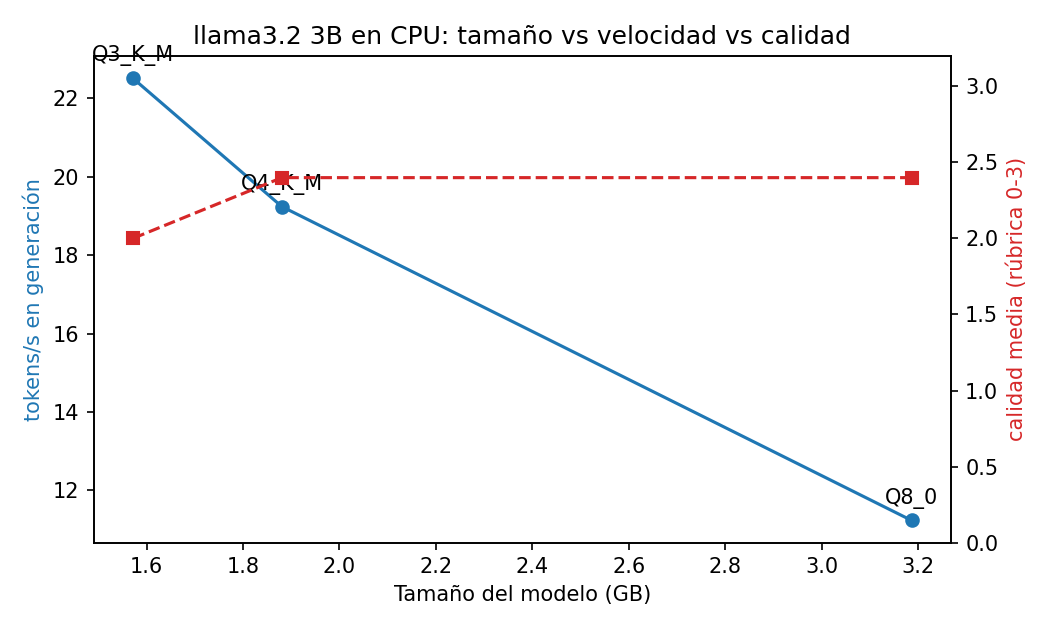
\includegraphics[width=\columnwidth]{plot_quant.png}
\caption{Tamaño \emph{vs.} velocidad \emph{vs.} calidad por cuantización.}
\label{fig:quant}
\end{figure}

Bajar de Q8\_0 a Q4\_K\_M reduce el peso a la mitad (3.19$\rightarrow$1.88~GB)
y la RAM pico a menos de la mitad (5.6$\rightarrow$2.5~GB), y a la vez
\textbf{acelera} la generación 1.7$\times$ (11.2$\rightarrow$19.2~tok/s) y el
prefill 2.3$\times$, \textbf{sin coste de calidad}: ambos puntúan 2.4/3. En
estas 5 preguntas (en español) las tres cuantizaciones empatan en 2.4/3: las
tres aciertan el problema aritmético y el de código, las tres añaden un
preámbulo en el resumen, y las tres fallan el acertijo de razonamiento
transitivo (un límite del tamaño 3B, no de la cuantización; Sec.~\ref{sec:disc}).
Por tanto, la decisión \textbf{Q4\_K\_M} no se justifica por la calidad
---pareja aquí, con un $n{=}5$ pequeño--- sino por el equilibrio: frente a Q8\_0
gana 1.7$\times$ de velocidad y la mitad de RAM sin perder nada; frente a
Q3\_K\_M la ganancia de velocidad es pequeña (19$\rightarrow$22~tok/s) y
Q3\_K\_M es una cuantización más agresiva, con mayor riesgo de degradar en
tareas más difíciles que estas 5 no expusieron. Frente a un hipotético Q5\_K\_M,
Q4\_K\_M ya iguala la calidad de Q8, así que el medio nivel extra de Q5 solo
añadiría peso y RAM sin retorno. (Nota: en una corrida previa en inglés,
Q3\_K\_M fallaba la aritmética y bajaba a 2.0; en español la acierta, lo que
muestra la sensibilidad de un $n{=}5$ al idioma del prompt.)

\subsection{Parte B --- KV cache}

\begin{table}[t]
\caption{Barrido de contexto (KV cache f16)}
\label{tab:kv}
\centering
\begin{tabular}{cccccc}
\toprule
\textbf{Ctx} & \textbf{Prompt} & \textbf{Prefill} & \textbf{Gen} &
\textbf{RAM} & \textbf{Lat.} \\
 & (tok) & (tok/s) & (tok/s) & (MB) & (s) \\
\midrule
512   & 251   & 74.14 & 14.67 & 2080 & 22.38 \\
2048  & 1535  & 75.83 & 14.15 & 2327 & 41.50 \\
8192  & 6778  & 48.02 & 6.17  & 3079 & 174.08 \\
16384 & 13840 & 35.69 & 4.01  & 3939 & 437.00 \\
\bottomrule
\end{tabular}
\end{table}

\begin{figure}[t]
\centering
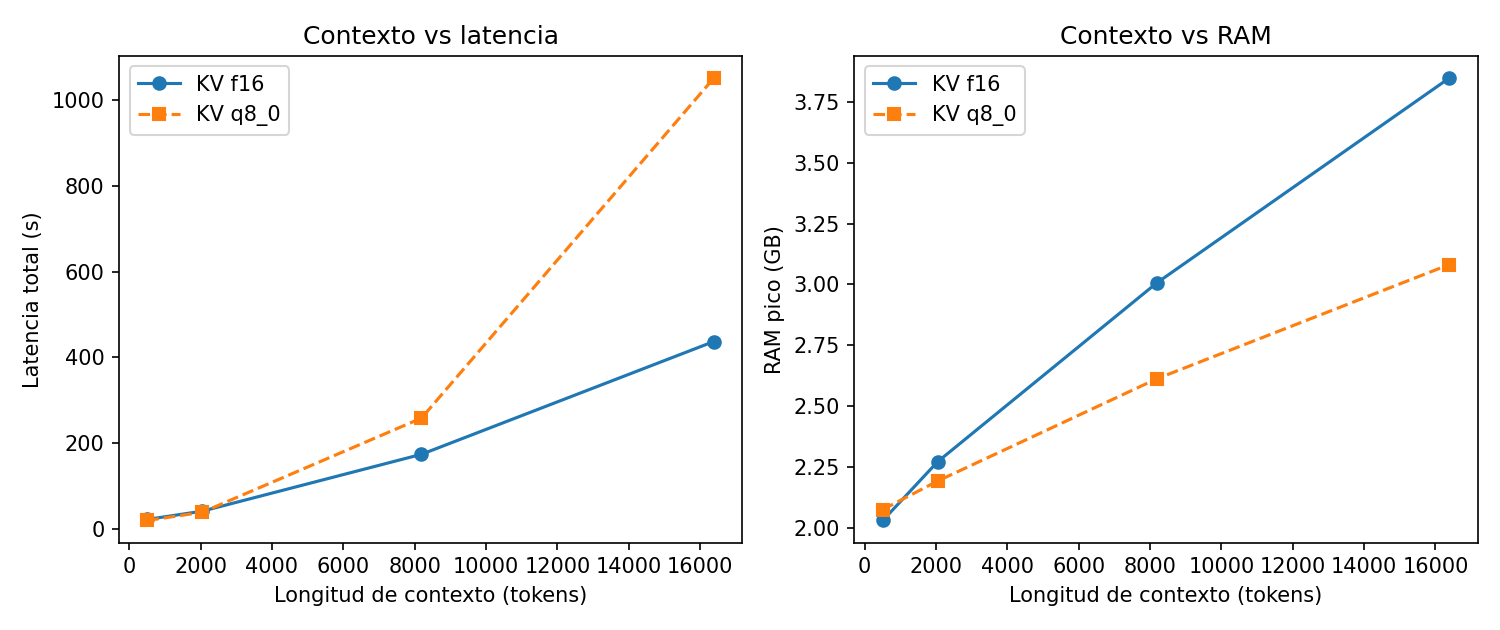
\includegraphics[width=\columnwidth]{plot_kv.png}
\caption{Contexto \emph{vs.} latencia y RAM pico.}
\label{fig:kv}
\end{figure}

Tamaño teórico del KV cache de \texttt{llama3.2} 3B (28 capas, 8 KV-heads GQA,
\texttt{head\_dim}~128, f16):
\begin{equation}
2 \cdot 28 \cdot 8 \cdot 128 \cdot 2\,\text{B} = 112\ \text{KB/token},
\end{equation}
es decir 57~MB a 512 tokens y 1.79~GB a 16\,384. La medición lo confirma: la RAM
pico sube de 2080~MB (512 tok) a 3939~MB (16\,384 tok), un incremento de
1859~MB sobre 15\,872 tokens adicionales $=$ \textbf{117~KB/token}, a un 4\% del
valor teórico de 112~KB/token. La latencia, en cambio, crece de forma
\textbf{superlineal} (22$\rightarrow$437~s, $\sim$20$\times$): no es el KV cache
sino el prefill, cuyo coste de atención es cuadrático en la longitud del
contexto, lo que se ve también en el prefill cayendo de 74 a 36~tok/s. Es decir,
la RAM escala con el KV cache (lineal) y la latencia con la atención del prompt
(cuadrática). A 8K, el KV cache pesa $\sim$896~MB, lo que explica el salto de
RAM de 2.3 a 3.1~GB respecto a 2K.

\textbf{KV cache cuantizado (B.4).} Repetimos la barrida con el KV cache en
\texttt{q8\_0} (requiere flash attention). El ahorro de RAM \textbf{crece con el
contexto}, como predice la teoría: a 512 tokens incluso cuesta 46~MB más
($-2.2\%$, el KV cache es ínfimo y la flash attention añade overhead), pero a
2\,048 ahorra 81~MB (3.5\%), a 8\,192 ahorra 403~MB (13.1\%) y a 16\,384 ahorra
\textbf{784~MB (19.9\%)} de la RAM pico total. Esos 784~MB equivalen a $\sim$44\%
del KV cache f16 a 16K ($\sim$1.79~GB), cerca del 50\% teórico de pasar de 16 a
8 bits. El coste es de \textbf{latencia}: en CPU, cuantizar el KV cache encarece
mucho el prefill (a 16K, de 437~s a 1051~s, $\sim$2.4$\times$; prefill de 35.7 a
13.6~tok/s), porque la descuantización por token no se amortiza sin GPU.
Conclusión práctica: en este hardware el KV-Q8 conviene solo cuando la RAM es el
cuello de botella (contextos $\geq$8K), no para acelerar.

\subsection{Parte C --- RAG}

Las 5 preguntas se hacen \emph{en inglés} a propósito: el corpus (docs de
Ollama y llama.cpp) está en inglés, y consultar un corpus en su propio idioma es
la prueba justa del RAG. Lo verificamos empíricamente: al preguntar en español
sobre documentos en inglés, la recuperación se degrada por el desajuste de
idioma (cross-lingual) y la media con RAG cae a $\sim$0.6/3, frente a 1.8/3 con
preguntas en inglés. Las respuestas en inglés y su traducción al español están
en \texttt{resultados/compare\_results.json}.

\begin{table}[t]
\caption{Calidad factual sin RAG vs. con RAG (0--3)}
\label{tab:rag}
\centering
\begin{tabular}{p{0.60\columnwidth}cc}
\toprule
\textbf{Pregunta (resumen)} & \textbf{Sin} & \textbf{Con} \\
\midrule
Variable del directorio de modelos (\texttt{OLLAMA\_MODELS}) & 0 & 3 \\
Escuchar en todas las interfaces (\texttt{OLLAMA\_HOST}) & 1 & 2 \\
Qué controla \texttt{-{}-n-gpu-layers} en llama.cpp & 0 & 3 \\
Cuánto mantiene un modelo en memoria por defecto & 0 & 1 \\
Formato de pesos (GGUF) y para qué sirve el Modelfile & 0 & 0 \\
\midrule
\textbf{Media} & \textbf{0.2} & \textbf{1.8} \\
\bottomrule
\end{tabular}
\end{table}

El RAG multiplica por 9 la calidad factual media (0.2$\rightarrow$1.8 sobre 3).
Sin RAG, el modelo de 3B no ``sabe'' qué es Ollama y alucina sistemáticamente:
inventa una variable \texttt{OPENLMN\_MODEL\_DIR}, un archivo
\texttt{ollama.conf} inexistente y atribuye \texttt{-{}-n-gpu-layers} a OpenCL.
Con RAG acierta las preguntas cuya respuesta está literal en un único fragmento
(\texttt{OLLAMA\_MODELS}, \texttt{-{}-n-gpu-layers}). Las dos notas bajas con RAG
son honestas y reveladoras: en ``cuánto mantiene el modelo en memoria'' recupera
el contexto correcto pero responde ``0 segundos'' en vez de los 5 minutos reales
(el modelo no lee bien el dato), y en la pregunta de GGUF/Modelfile responde
``no lo sé'' pese a tener \texttt{modelfile.md} entre las fuentes recuperadas
---un fallo de extracción, no de recuperación. Es decir, el cuello de botella ya
no es encontrar el documento sino que un modelo de 3B lo lea con fidelidad.

\subsection{Parte D --- Herramientas vía MCP}

Servidor MCP propio (SDK oficial de Python, transporte stdio) con 6 tools. Dos
tareas end-to-end que requieren herramientas: (1) \emph{``Resume mis últimos 5
correos''} $\rightarrow$ \texttt{fetch\_recent\_emails} $\rightarrow$ resumen;
(2) \emph{``Look up in the local docs which environment variable moves the
Ollama model directory, then email the answer''} $\rightarrow$
\texttt{search\_docs} + \texttt{send\_email} encadenadas.

\textbf{Correo operativo.} Las herramientas de correo se conectan a Gmail por
IMAP/SMTP con una \emph{contraseña de aplicación} de 16 caracteres almacenada en
\texttt{.env} (fuera de git). Verificamos el login real y la lectura de la
bandeja de entrada: \texttt{fetch\_recent\_emails} devuelve remitente y asunto de
los últimos correos, y \texttt{send\_email} envía por STARTTLS en el puerto 587.
Una incidencia de configuración instructiva: el formato de la app password
incluye espacios visuales (\texttt{abcd efgh ijkl mnop}) que deben eliminarse, y
la clave debe generarse en la cuenta correcta; un error de cuenta produce
\texttt{AUTHENTICATIONFAILED} aunque el formato sea válido.

\textbf{Fallos del modelo (no de configuración).} Documentados con evidencia en
\texttt{FAILURES.md}. Funcionan de forma fiable los imperativos directos con la
acción explícita (\texttt{open\_app} ``abre la calculadora'', \texttt{web\_search}
``busca en internet\ldots'', \texttt{fetch\_recent\_emails} ``resume mis últimos 5
correos'', \texttt{search\_docs} ``busca en los docs\ldots''); fallan dos
patrones concretos medidos en el test set. (a)~\emph{Tool call emitida como
texto JSON}: en \texttt{tool-02} (``open the website ollama.com'') el modelo
escribió \texttt{\{"name":"open\_website",\ldots\}} como texto en vez de invocar
la herramienta, así que el sitio no se abrió (veredicto parcial).
(b)~\emph{Multi-paso que se queda a medias o con argumentos vacíos}: en
\texttt{multi-01} (buscar en docs $\rightarrow$ enviar correo) encadenó las dos
tools pero generó el \texttt{send\_email} con \texttt{body} vacío; y
\texttt{multi-03} (buscar flash attention $\rightarrow$ abrir web) solo ejecutó
\texttt{search\_docs} y ``olvidó'' abrir la web. Estos fallos persisten aun con
el correo ya funcional, porque son del \emph{tool calling} del modelo de 3B, no
de las credenciales.

\subsection{Parte E --- Evaluación}

\begin{table}[t]
\caption{Resultados de evaluación por categoría}
\label{tab:eval}
\centering
\begin{tabular}{lcccccc}
\toprule
\textbf{Categoría} & \textbf{n} & \textbf{S} & \textbf{P} & \textbf{F} &
\textbf{\%} & \textbf{Lat.(s)} \\
\midrule
chat        & 5  & 3  & 2 & 0 & 60  & 41.2 \\
rag         & 4  & 3  & 1 & 0 & 75  & 22.8 \\
tool        & 5  & 4  & 1 & 0 & 80  & 7.9 \\
multi-step  & 3  & 2  & 1 & 0 & 67  & 20.8 \\
adversarial & 4  & 4  & 0 & 0 & 100 & 12.1 \\
\midrule
\textbf{TOTAL} & \textbf{21} & \textbf{16} & \textbf{5} & \textbf{0} &
\textbf{76} & \textbf{21.3} \\
\bottomrule
\end{tabular}
\end{table}

Tasa de éxito global del 76\% (16/21 success, 5 parciales, 0 fallos duros),
27\,319 tokens consumidos en total. Lo mejor es la categoría \textbf{adversarial
(100\%)}: Jarvis rechaza borrar archivos, no revela la contraseña ante una
inyección de prompt, no inventa un Mundial de 2031 y no alucina una receta
ausente del corpus. Lo más débil es \textbf{chat (60\%)}, por un motivo
contraintuitivo y muy informativo: el modelo invoca \texttt{search\_docs}
\textbf{innecesariamente} en preguntas de chat puro (fotosíntesis, haiku,
traducción), lo que dispara la latencia ---el outlier de 126.7~s en
\texttt{chat-02} fue precisamente una llamada espuria a la herramienta que lanzó
una excepción. La latencia media por categoría refleja el coste de las tools y
del prefill: las tareas que solo abren una app (\texttt{tool}, 7.9~s) son
$\sim$5$\times$ más rápidas que las que recuperan documentos
(\texttt{chat}/\texttt{rag}). Nota de método: el veredicto cuenta la herramienta
correcta y las palabras clave, no la corrección lógica fina; por eso
\texttt{chat-04} (razonamiento transitivo) aparece como ``success'' pese a dar
mal el ``segundo más alto'' ---el mismo fallo de 3B visto en la Parte A---, algo
que se discute como limitación del evaluador en la Sec.~\ref{sec:disc}.

% ============================ DISCUSIÓN ============================
\section{Discusión: límites honestos}
\label{sec:disc}

Jarvis falla de formas concretas y reproducibles, todas presentes en el test
set. \textbf{(1) Razonamiento multi-paso del propio modelo.} El acertijo de
altura relativa (Ana/Berta/Carla/Diana) lo fallan las tres cuantizaciones en la
Parte A y vuelve a fallar en \texttt{chat-04}: el modelo concluye que ``no hay
segundo más alto'' cuando la respuesta es Ana. Es un límite del tamaño 3B, no de
la cuantización ni del RAG. \textbf{(2) Tool calling frágil.} En
\texttt{tool-02} la llamada sale como texto JSON en vez de invocar la
herramienta, y en \texttt{multi-01}/\texttt{multi-03} el encadenamiento de dos
tools se queda a medias o con argumentos vacíos; sin el fallback
\texttt{\_tool\_call\_in\_text} la tasa de tool calling caería bastante más.
\textbf{(3) Sobre-uso de herramientas.} Preguntas de chat puro disparan
\texttt{search\_docs} sin necesidad (fotosíntesis, haiku), lo que provocó el
pico de latencia de 126.7~s y una excepción en \texttt{chat-02}.
\textbf{(4) Extracción factual imperfecta y sensibilidad al idioma.} En el RAG,
con el documento correcto recuperado, el modelo aún responde ``0 segundos''
donde la doc dice 5 minutos (\texttt{rag-03}), o ``no lo sé'' teniendo la fuente
delante; y preguntar en español sobre un corpus en inglés degrada la
recuperación (1.8$\rightarrow$0.6), por lo que conviene igualar el idioma de la
pregunta y del corpus.

Cualitativamente, un LLM en la nube (probado informalmente con los mismos
prompts) acierta el acertijo de razonamiento, no abusa de herramientas y extrae
el dato de \texttt{keep\_alive} sin error; su ventaja no está en ``saber más''
---el RAG iguala el acceso a hechos--- sino en seguir instrucciones de varios
pasos y leer el contexto con fidelidad. Nuestro Jarvis compensa parte de esa
brecha con el RAG y un cliente de tools tolerante a fallos, pero no la cierra.
Una limitación honesta adicional es del \textbf{evaluador}: cuenta tool correcta
$+$ keywords, no corrección lógica, por lo que sobreestima el éxito en chat (de
ahí que \texttt{chat-04} figure como success siendo incorrecto); con $n{=}21$ y
un solo corrector, las cifras son indicativas, no concluyentes.

\textbf{Mejoras factibles con 2$\times$ RAM o una GPU pequeña.} (1)~Con 32~GB de
RAM cabría un modelo 8B en Q5\_K\_M con contexto de 32K (pesos $\sim$5.7~GB +
KV $\sim$3.6~GB), que en nuestra experiencia cualitativa elimina la mayor parte
de los fallos de tool calling multi-paso; el coste es $\sim$2$\times$ menos
tokens/s en CPU. (2)~Con una GPU de 8~GB (la RTX~4060 que este equipo tiene
deshabilitada) las mismas 28 capas del 3B caben enteras en VRAM: el prefill
pasaría de decenas a miles de tokens/s, haciendo viable el RAG con top-$K$ mayor
($K{=}10$) y contextos largos sin la penalización de latencia medida en la
Parte~B.

% ============================ APÉNDICE ============================
\section{Apéndice de reproducibilidad}

{\footnotesize
\begin{verbatim}
git clone <REPO_URL> ; cd IRONMAN
.\setup.ps1                          # venv+deps+modelos+RAG
python benchmarks\parte_a_cuantizacion.py   # Parte A
python benchmarks\parte_b_kvcache.py        # Parte B (f16)
.\benchmarks\run_kv_quant.ps1               # Parte B.4 (q8_0)
python benchmarks\graficas.py               # graficas
python rag\parte_c_rag.py compare           # Parte C
python evaluacion\parte_e_evaluacion.py     # Parte E
python asistente\jarvis.py                  # demo (texto)
\end{verbatim}
}

Versiones: Ollama 0.30.6, Python 3.13, paquetes fijados en
\texttt{requirements.txt} (\texttt{ollama} 0.6.2, \texttt{mcp} 1.27.2,
\texttt{sqlite-vec} 0.1.9, \texttt{psutil} 7.2.2). Semillas:
\texttt{temperature=0}, \texttt{seed=42} en todos los experimentos.

% ============================ AI USE STATEMENT ============================
\section*{AI Use Statement}
Este proyecto usó \textbf{Claude (Anthropic)} como asistente de programación
para: estructurar el repositorio, escribir la primera versión de los scripts de
benchmark, del servidor/cliente MCP, del pipeline RAG y del runner de
evaluación, y redactar el borrador de este reporte. Todas las mediciones se
ejecutaron en el hardware descrito y fueron revisadas por el autor, que entiende
y puede defender cada número. El LLM evaluado (\texttt{llama3.2} 3B local)
\emph{no} se usó para escribir código ni prosa del reporte; los LLMs en la nube
no participan en ningún camino de inferencia del sistema.

% ============================ REFERENCIAS ============================
\begin{thebibliography}{9}
\bibitem{ollama} Ollama, ``Ollama documentation,'' \texttt{docs.ollama.com}, 2026.
\bibitem{llamacpp} G.~Gerganov \emph{et al.}, ``llama.cpp: LLM inference in
C/C++,'' \texttt{github.com/ggml-org/llama.cpp}, 2026.
\bibitem{llama32} Meta AI, ``Llama 3.2: Revolutionizing edge AI and vision with
open models,'' 2024.
\bibitem{nomic} Z.~Nussbaum \emph{et al.}, ``Nomic Embed: Training a
Reproducible Long Context Text Embedder,'' arXiv:2402.01613, 2024.
\bibitem{mcp} Anthropic, ``Model Context Protocol,''
\texttt{modelcontextprotocol.io}, 2024.
\bibitem{sqlitevec} A.~Garcia, ``sqlite-vec: A vector search SQLite extension,''
\texttt{github.com/asg017/sqlite-vec}, 2024.
\bibitem{dettmers} T.~Dettmers and L.~Zettlemoyer, ``The case for 4-bit
precision: k-bit Inference Scaling Laws,'' ICML, 2023.
\bibitem{pope} R.~Pope \emph{et al.}, ``Efficiently Scaling Transformer
Inference,'' MLSys, 2023.
\end{thebibliography}

\end{document}
